\documentclass[uplatex,dvipdfmx]{jsarticle}

\usepackage[uplatex,deluxe]{otf} 
\usepackage[noalphabet]{pxchfon} 
\usepackage{stix2} 
\usepackage[fleqn,tbtags]{mathtools} 
\usepackage{amsmath}
\usepackage{url}
\usepackage{float}
\usepackage{xurl}
\usepackage{graphicx}

\begin{document}

\title{システム設計書}
\author{25G1051 近藤巧望}
\date{\today}
\maketitle

\section{\textbf{システムの基本設計}}

\subsection{\textbf{機能一覧}}
\begin{itemize}
    \item \textgt{テンポ同期機能：} 
        PCブラウザ上で入力されたテンポ（BPM）情報を，マスター機を介して受信し，ユニット内部の演奏速度をリアルタイムに同期させる機能である．
    \item \textgt{自動演奏機能：} 
        同期されたテンポに基づき，プログラム済みのメロディデータを正確なタイミングで再生する機能である．
    \item \textgt{外部連携合図送信機能：} 
        演奏の開始タイミングに合わせて，Processingへ再生開始の合図（トリガー）とテンポ情報を送信し，伴奏音源との同期を確立する機能である．
\end{itemize}

\subsection{\textbf{システム構成図}}
トロンボーンのシステム構成を図\ref{fig:system_kousei}に示す．
\begin{center}
\begin{figure}[H]
        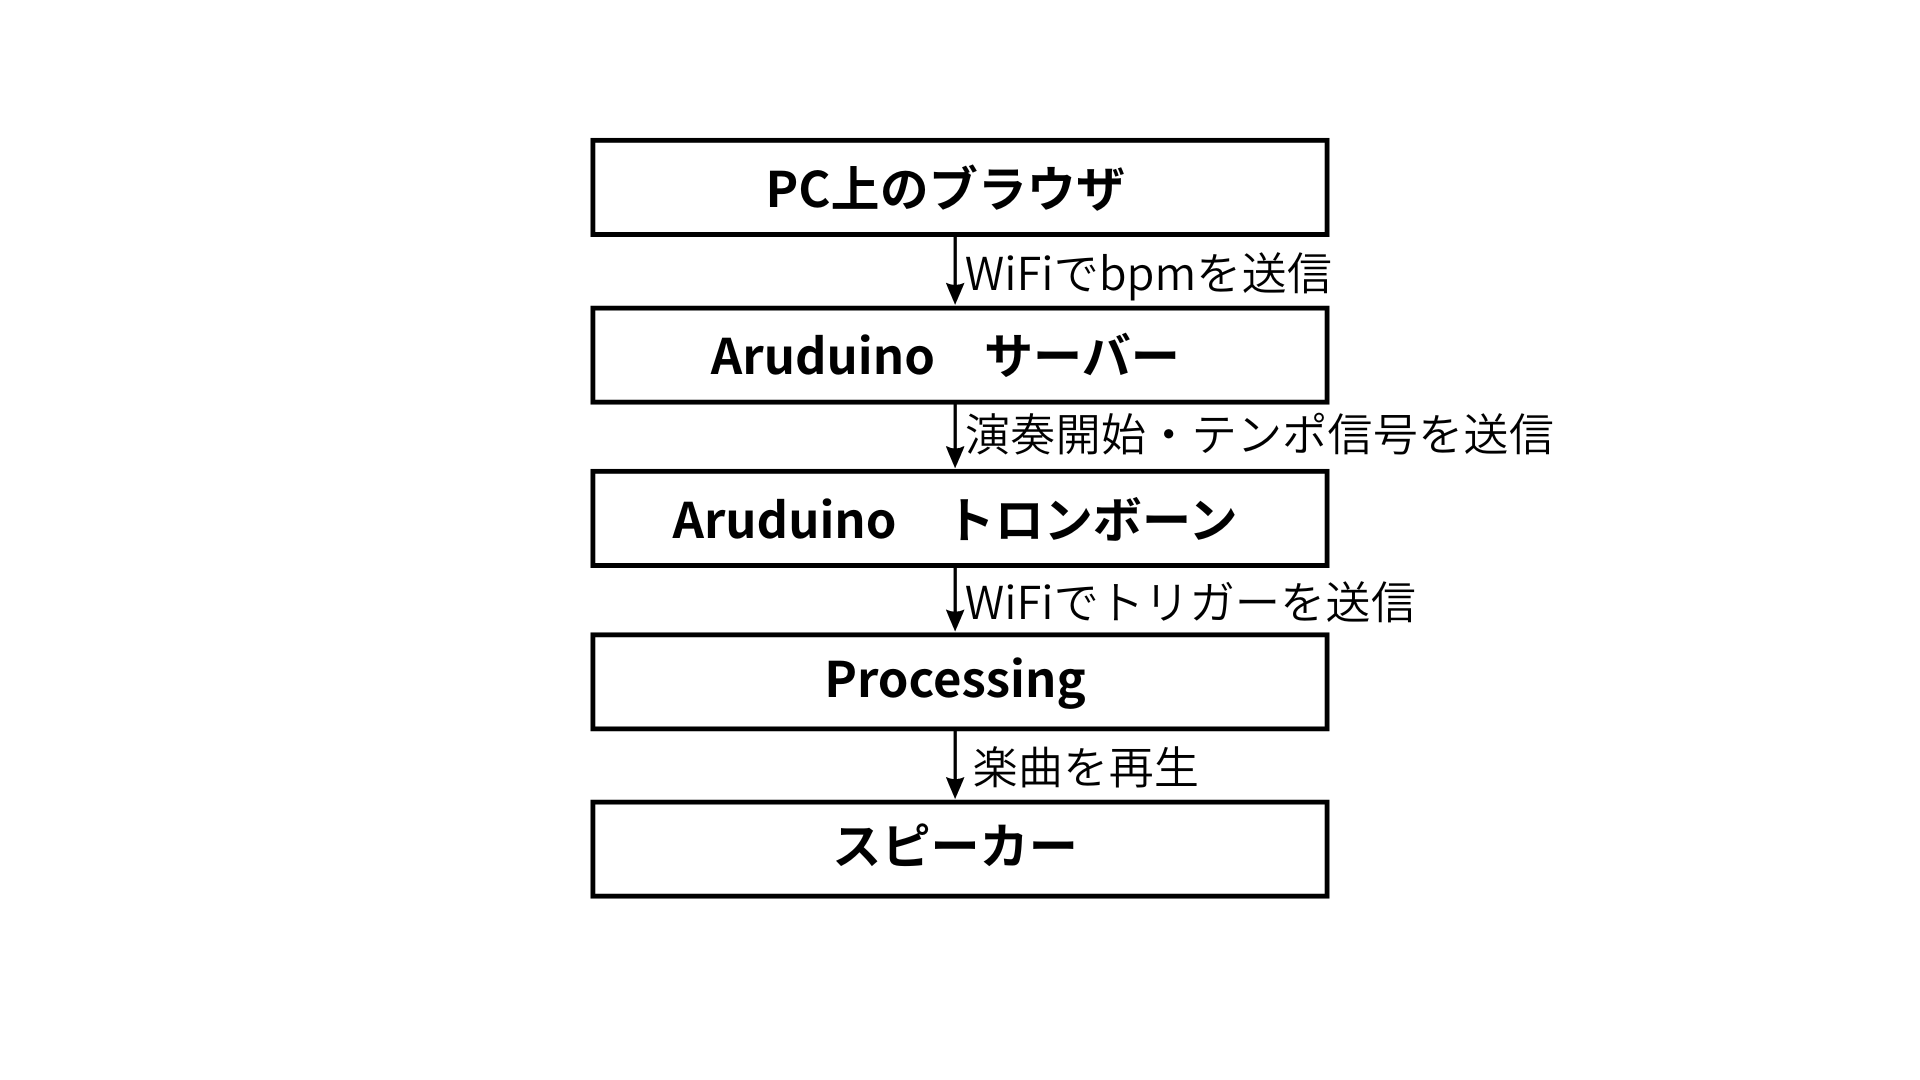
\includegraphics[width=1.0\textwidth]{system_kousei.png}
        \caption{トロンボーン部分のシステム構成図}
        \label{fig:system_kousei}
\end{figure}
\end{center}

\subsection{\textbf{操作インターフェース設計}}
Web Serial APIを利用したブラウザUI（接続・BPM入力・送信）を実装する．

\subsection{\textbf{状態遷移図}}
本ユニットは，外部機器との同期を自動的に行うため，接続および同期の進捗状況に基づき図\ref{joutai}の通り遷移する．
\begin{center}
\begin{figure}[H]
        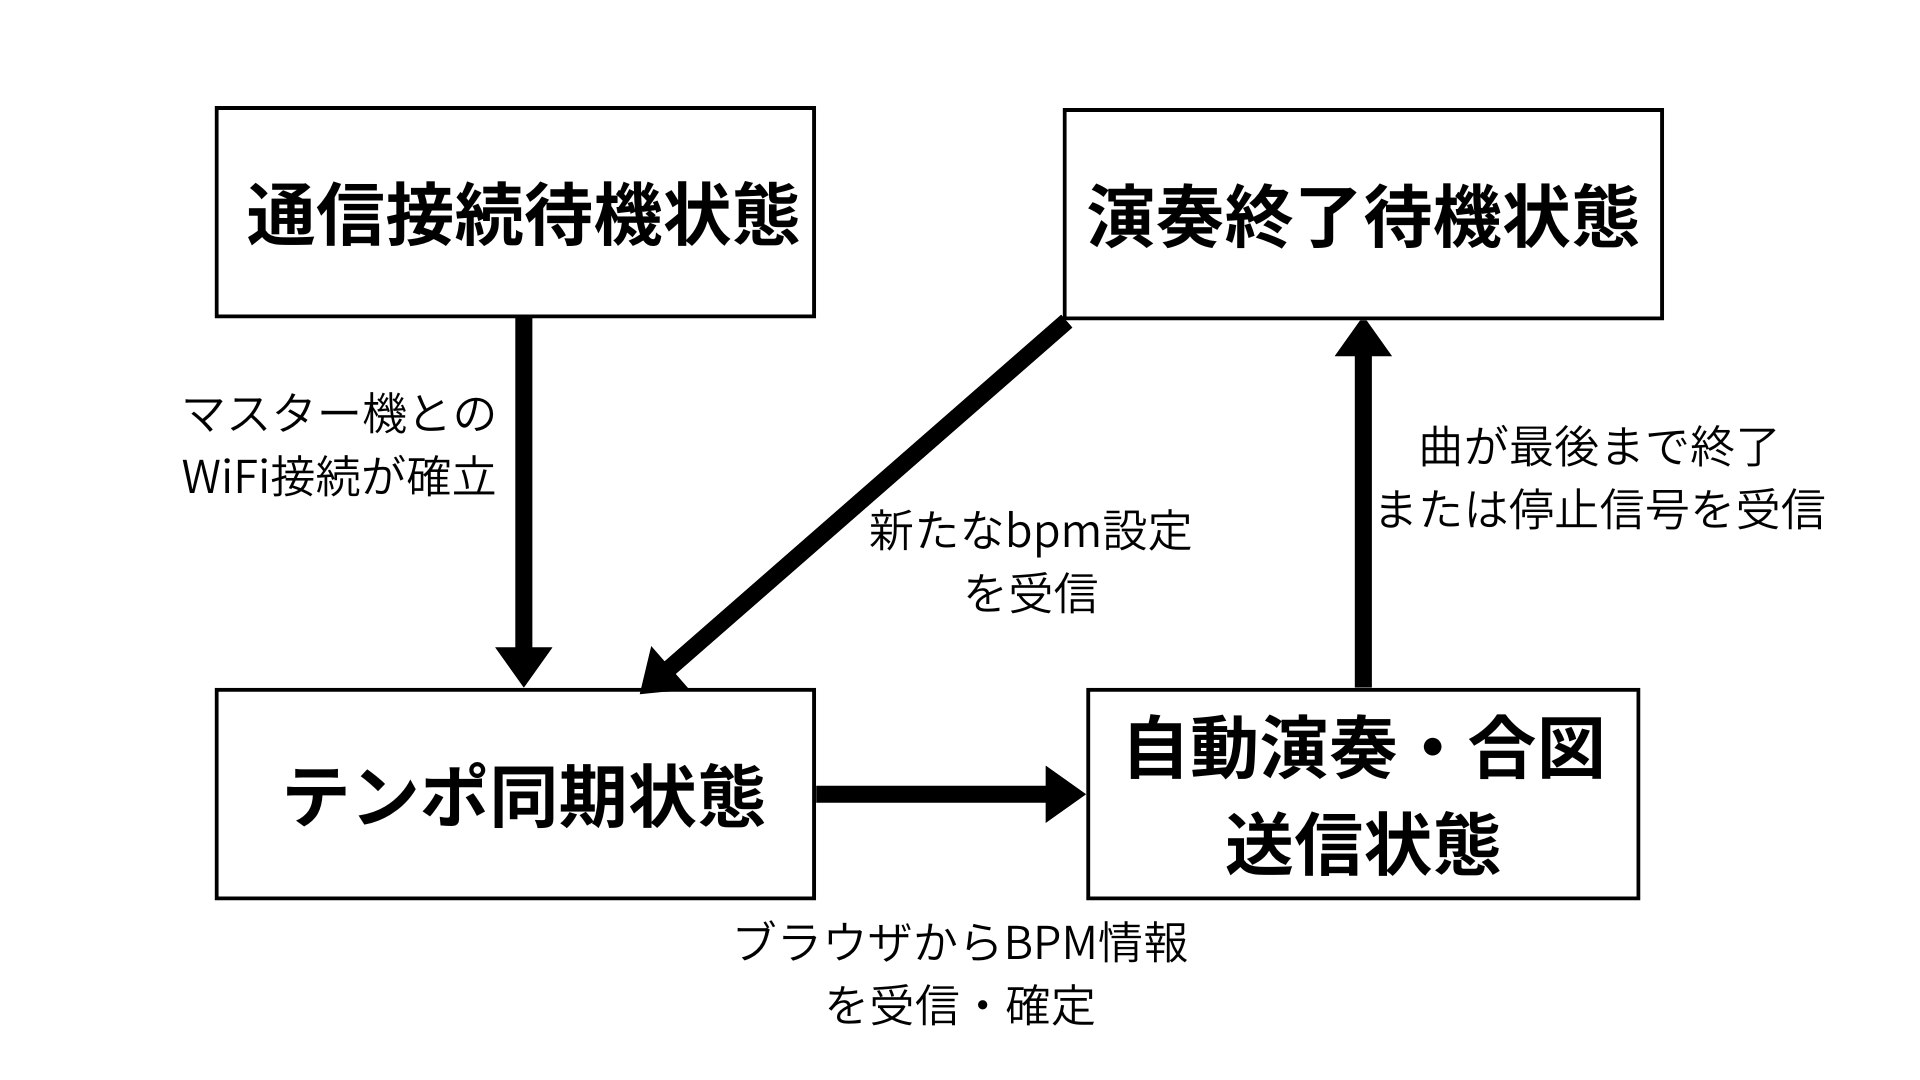
\includegraphics[width=1.0\textwidth]{joutai.png}
        \caption{トロンボーン部分の状態遷移図}
        \label{joutai}
\end{figure}
\end{center}

また，図\ref{joutai}の状態遷移において，各状態の役割は以下の通りである．

\begin{itemize}
\item \textgt{1．通信接続待機状態（待機）：}
電源投入直後の初期状態である．マイコンがWiFiネットワークへ接続し，マスター機からの信号を受け入れ可能になるまで待機する．ネットワークの確立が確認されると，自動的に次の状態へ遷移する．
\item \textgt{2．テンポ同期状態（準備）：}
ブラウザUIから送信されるWeb OSCメッセージ（BPM情報）を待機・受信する状態である．受信した数値に基づき，ユニット内部の演奏タイマーをマスター機の基準クロックにミリ秒単位で一致させる．テンポの確定が遷移のトリガーとなる．
\item \textgt{3．自動演奏・合図送信状態（実行）：}
テンポ確定と同時に移行するメインの状態である．プログラムされた音階データを再生しつつ，第1拍目の瞬間にProcessingへ開始合図（トリガー）を送信する．これにより，楽器演奏と伴奏の完全な同時スタートが保証される．
\item \textgt{4．演奏終了待機状態（停止）：}
楽曲データの再生が完了した，あるいはブラウザから停止命令を受信した際の状態である．音出力を停止し，システムを初期化する．新たなテンポ設定を受信することで，再び「2．テンポ同期状態」へと戻る．
\end{itemize}

\section{\textbf{システムの詳細設計}}

\subsection{\textbf{部品一覧}}
本ユニットを構成する主要な要素を以下に示す．
\begin{itemize}
\item \textgt{通信制御マイコン（Arduino Uno R4 WiFi）：} 通信・制御を一体で行う主機．内蔵の無線通信機能により，外部デバイスとのデータ交換を行う．
\item \textgt{PC（Processing動作環境）：} 全体の伴奏音源およびトロンボーン演奏音の出力（スピーカー）を担当する．
\end{itemize}

%\subsection{ハードウェア設計}


\subsection{\textbf{ソフトウェア設計}}

\subsubsection{\textbf{ファイル構成}}
\begin{itemize}
\item \texttt{Main.ino}：メインループおよびシステム全体の動作状態管理．
\item \texttt{OscParser.cpp / .h}：受信したWeb OSCメッセージ（BPM，開始合図）の解析．
\item \texttt{AudioEngine.cpp / .h}：BPMに同期したタイマー管理および音響生成ロジック．
\item \texttt{NetworkConfig.h}：WiFi接続情報および外部同期先のIPアドレス定義．
\end{itemize}

\subsubsection{\textbf{オブジェクト設計（クラス図）}}
\begin{itemize}
\item \textgt{BpmReceiverクラス：} ブラウザから送信されたBPM値を取得し，システム変数へ反映する．
\item \textgt{PlayManagerクラス：} 自動演奏のタイミング制御およびメロディデータの読み出しを行う．
\item \textgt{SyncSenderクラス：} 演奏開始と同時にProcessing宛てのOSCパケットを構築・送出する．
\end{itemize}

\subsubsection{\textbf{関数設計}}
\begin{itemize}
\item \texttt{void receiveBpm()}：UDPポートを監視し，BPM値が含まれるパケットを受信した際に内部数値を更新する．
\item \texttt{void updateTimerInterval(float bpm)}：BPMをタイマー割り込み周期へ変換し，ハードウェアレジスタへ即座に反映する．
\item \texttt{void broadcastTrigger()}：演奏の第1拍目に合わせ，無線ネットワーク経由で開始合図を射出する．
\end{itemize}

\subsection{\textbf{処理フローの設計}}
本システムは，以下の3段階の自動化フローによって動作する．
\begin{enumerate}
\item \textgt{初期化：} 起動時にWiFi接続を確立し，外部からのOSCパケット受信を待機する．
\item \textgt{同期：} ブラウザUIでの操作（BPM確定）を受け，内部の演奏タイマーをマスター機と同期させる．
\item \textgt{実行：} 確定したテンポで自動演奏を開始し，同時にProcessingへ向けて「演奏開始合図」を自動送信する．
\end{enumerate}

また，図\ref{flow}に処理フローの概要を示す．
\begin{center}
\begin{figure}[H]
        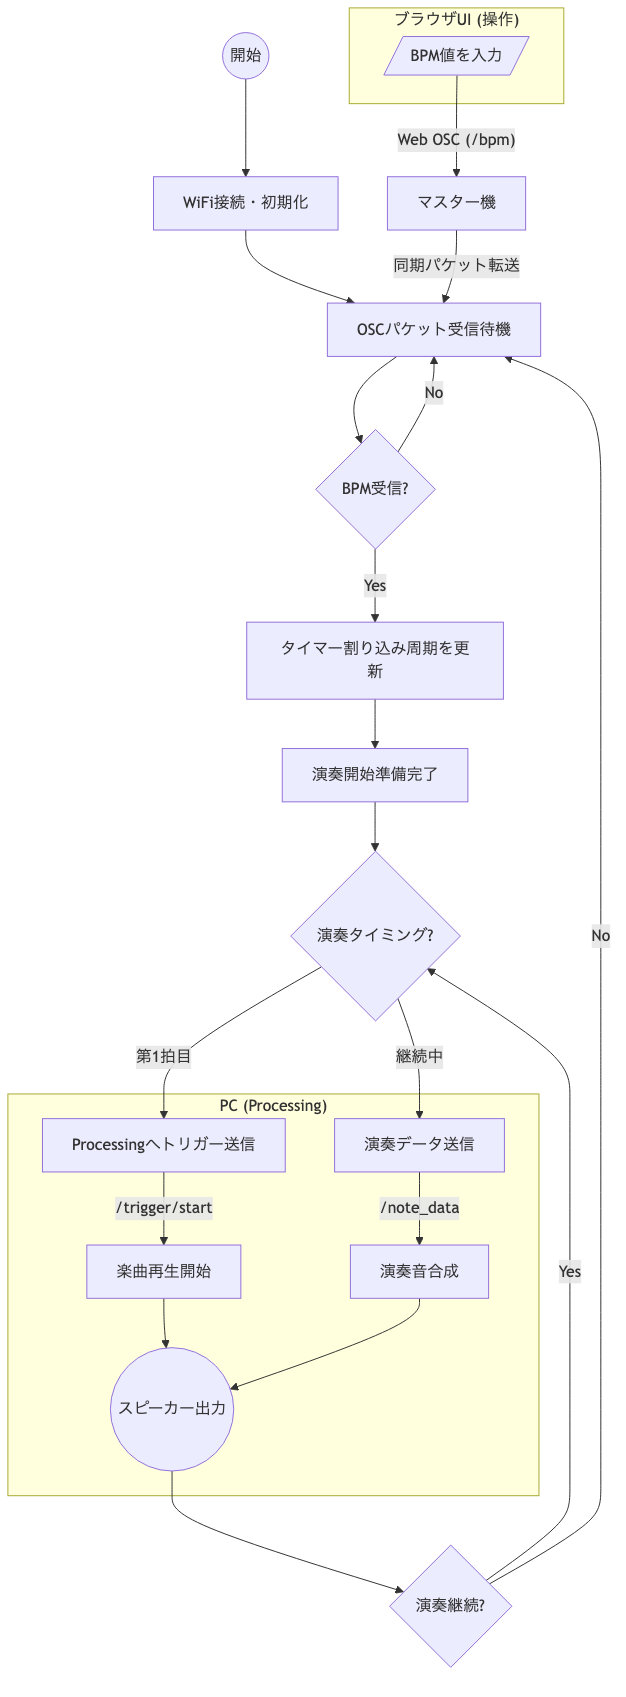
\includegraphics[width=0.5\textwidth]{flow.png}
        \caption{トロンボーン部分の処理フロー図}
        \label{flow}
\end{figure}
\end{center}

\subsection{\textbf{テストの設計}}
\begin{itemize}
\item \textgt{データ整合性テスト：} ブラウザ上で入力したBPM値が，トロンボーン側で正確な演奏周期として反映されているかを確認する．
\item \textgt{同時再生テスト：} トロンボーンの第1拍目の発音と，Processing側の伴奏再生の開始が完全に一致するかを確認する．
\item \textgt{非接触制御テスト：} 物理的な接点を一切持たず，ネットワーク経由のデータ通信のみで一連の動作が完結することを確認する．
\end{itemize}

\end{document}